% chapters/thygate.tex
% generated from thyristor_gate_driver.tex
\chapter{Thyristor gate driver design guidelines}
\label{ch:thygate}
\begin{chapabstract}
\noindent
This note collects the practical requirements that govern the design of a gate
driver (gate unit) for phase-control and line-commutated thyristors, from small
stud-mount devices up to large press-pack SCRs used in \si{\mega\watt}-class
rectifiers and soft starters. The gate--cathode characteristic and the datasheet
limits are reviewed first, followed by the requirements on pulse amplitude, slope,
duration and off-state bias. Isolation, auxiliary supply, protection, layout and
diagnostics are then treated. Four representative driver topologies are proposed
and discussed, and a worked numerical example is given for a
\SI{6.5}{\kilo\volt}/\SI{2.6}{\kilo\ampere} press-pack device. The document closes
with a design checklist.
\end{chapabstract}

%======================================================================
\section{Scope and Terminology}
%======================================================================

The subject of this note is the \emph{gate unit}: the electronic circuit that
converts a logic-level firing command, referenced to the control ground, into a
gate current pulse referenced to the cathode of a thyristor floating at line
potential.

Three functions are always present and should be designed separately:

\begin{enumerate}[label=(\roman*)]
  \item \textbf{Signal isolation} --- transferring the firing command across the
        insulation barrier without distortion and with adequate common-mode
        transient immunity.
  \item \textbf{Energy delivery} --- sourcing the gate charge with the required
        amplitude, slope and duration.
  \item \textbf{Protection and off-state control} --- keeping the device firmly
        off when no command is present, and preventing spurious triggering.
\end{enumerate}

The note is written for \emph{phase-control thyristors} (PCT) and
\emph{fast/inverter-grade thyristors} that are turned off by circuit commutation.
Gate-turn-off devices (GTO, IGCT) are outside the scope: they require a
fundamentally different, low-inductance turn-off path and are covered by dedicated
literature. Light-triggered thyristors (LTT) are mentioned only where relevant for
the isolation discussion.

%======================================================================
\section{The Gate: Physical Behaviour and Datasheet Parameters}
%======================================================================

\subsection{The gate--cathode junction}

Electrically, the gate--cathode path is a large-area, heavily interdigitated
$p$--$n$ junction shunted by the distributed emitter short-circuit structure of the
cathode. It therefore behaves as a diode in parallel with a resistance, with a
strongly non-linear $I_G$--$V_G$ characteristic and a wide unit-to-unit spread. It
is \emph{not} a capacitive load like a MOSFET or IGBT gate: the driver must deliver
sustained current, not just charge.

Triggering occurs when the injected gate current raises the current gain of the
$npn$ section far enough to satisfy the regenerative condition
$\alpha_{pnp}+\alpha_{npn}\ge 1$ in the region adjacent to the gate. Conduction
then \emph{spreads laterally} from that region at a plate velocity of the order of
\SIrange{50}{100}{\micro\metre\per\micro\second}. This spreading phenomenon is the
physical reason why the gate pulse shape, and not only its amplitude, determines
the tolerable anode $\mathrm{d}i/\mathrm{d}t$.

\subsection{The trigger diagram}

The datasheet parameters that define the required driver output characteristic are:

\begin{description}[style=nextline,leftmargin=2.2cm,labelwidth=2cm]
  \item[$V_{GT}$, $I_{GT}$] Gate trigger voltage and current: the values that
        guarantee firing, specified at \SI{25}{\celsius} and often also at
        $T_{vj,\min}$.
  \item[$V_{GD}$, $I_{GD}$] Gate non-trigger voltage and current: the values below
        which the device is guaranteed \emph{not} to fire, specified at
        $T_{vj,\max}$. The driver output in the off state must stay below these
        values with margin.
  \item[$I_L$, $I_H$] Latching and holding current. The gate pulse must last until
        the anode current has exceeded $I_L$.
  \item[$V_{FGM}$, $I_{FGM}$] Peak forward gate voltage and current.
  \item[$V_{RGM}$] Peak reverse gate voltage --- typically only
        \SIrange{5}{10}{\volt}. This is the most frequently violated limit in
        practice.
  \item[$P_{GM}$, $P_{G(AV)}$] Peak and average gate power dissipation, the latter
        usually specified over a \SI{20}{\milli\second} window.
\end{description}

Plotting these limits on the $V_G$--$I_G$ plane produces the classical trigger
diagram of Fig.~\ref{thygate:fig:trigger}. The design rule is simple to state:

\begin{quote}
\emph{The load line of the gate driver, drawn on the trigger diagram, must pass
entirely through the ``certain firing'' area over the whole operating temperature
range, and must never cross the $P_{GM}$, $V_{FGM}$ or $I_{FGM}$ boundaries.}
\end{quote}

\begin{figure}[htbp]
\centering
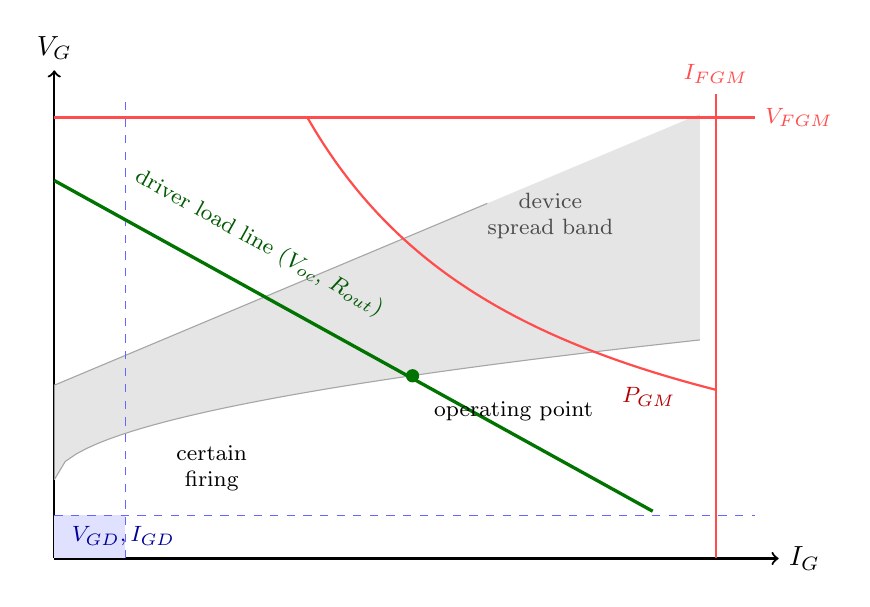
\begin{tikzpicture}[scale=1.0]
  % axes
  \draw[->,thick] (0,0) -- (9.2,0) node[right] {$I_G$};
  \draw[->,thick] (0,0) -- (0,6.2) node[above] {$V_G$};

  % device characteristic spread band
  \fill[gray!20]
    plot[domain=0:8.2,samples=60] (\x,{1.0+0.62*sqrt(\x)})
    -- (8.2,{2.2+0.42*8.2}) -- plot[domain=8.2:0,samples=60] (\x,{2.2+0.42*\x})
    -- cycle;
  \draw[gray!70] plot[domain=0:8.2,samples=60] (\x,{1.0+0.62*sqrt(\x)});
  \draw[gray!70] plot[domain=0:5.5,samples=60] (\x,{2.2+0.42*\x});
  \node[gray!60!black,align=center,font=\footnotesize]
    at (6.3,4.35) {device\\spread band};

  % non-trigger region
  \fill[blue!12] (0,0) rectangle (0.9,0.55);
  \draw[blue!60,dashed] (0.9,0) -- (0.9,5.9);
  \draw[blue!60,dashed] (0,0.55) -- (8.9,0.55);
  \node[blue!60!black,font=\footnotesize,anchor=west] at (0.05,0.28)
    {\,$V_{GD},I_{GD}$};

  % max limits
  \draw[red!70,thick] (8.4,0) -- (8.4,5.9) node[above,font=\footnotesize] {$I_{FGM}$};
  \draw[red!70,thick] (0,5.6) -- (8.9,5.6) node[right,font=\footnotesize] {$V_{FGM}$};
  % power hyperbola  V*I = 18
  \draw[red!70,thick] plot[domain=3.22:8.4,samples=60] (\x,{18/\x});
  \node[red!70!black,font=\footnotesize] at (7.55,2.05) {$P_{GM}$};

  % driver load line
  \draw[very thick,green!45!black] (0,4.8) -- (7.6,0.6);
  \node[green!35!black,font=\footnotesize,rotate=-29] at (2.6,4.0)
    {driver load line ($V_{oc}$, $R_{out}$)};
  \fill[green!45!black] (4.55,2.32) circle (2.4pt);
  \node[font=\footnotesize,anchor=north west] at (4.7,2.12) {operating point};

  % certain firing region label
  \node[align=center,font=\footnotesize] at (2.0,1.15)
    {certain\\firing};
\end{tikzpicture}
\caption{Thyristor gate trigger diagram. The driver load line must intersect the
device spread band inside the certain-firing area and stay below the $P_{GM}$,
$V_{FGM}$ and $I_{FGM}$ boundaries. The blue region is the guaranteed
non-triggering area at $T_{vj,\max}$.}
\label{thygate:fig:trigger}
\end{figure}

\subsection{Temperature and spread}

Two effects dominate the sizing:

\begin{itemize}
  \item $I_{GT}$ \textbf{increases at low temperature}, typically by a factor of
        \numrange{2}{4} between \SI{25}{\celsius} and \SI{-40}{\celsius}, because
        the emitter shorts divert a larger fraction of the gate current at low
        carrier lifetime. \textbf{The driver must be dimensioned at
        $T_{vj,\min}$}, i.e.\ for cold start-up, not at rated junction temperature.
  \item $V_{GD}$ and $I_{GD}$ \textbf{decrease at high temperature}. The off-state
        margin must therefore be verified at $T_{vj,\max}$.
\end{itemize}

Unit-to-unit spread on $I_{GT}$ within one production type is commonly a factor of
three or more. Designing for the typical value is a guaranteed field failure; the
datasheet maximum at the minimum operating temperature is the correct starting
point.

%======================================================================
\section{Requirements for the Gate Pulse}
%======================================================================

\subsection{Amplitude: hard firing}

The minimum requirement is $I_G > I_{GT}(T_{vj,\min})$, but this is never used in
practice. The accepted design rule is

\begin{equation}
  I_{G,\text{peak}} \;\ge\; 3 \dots 10 \times I_{GT}\big(T_{vj,\min}\big),
  \label{thygate:eq:amp}
\end{equation}

with the upper end of the range used whenever high anode $\mathrm{d}i/\mathrm{d}t$
is expected. The reason is the lateral spreading mechanism: a large gate current
turns on a larger initial cathode area, so the initial current density --- and
therefore the local dissipation during the first microseconds --- is lower. The
$\mathrm{d}i/\mathrm{d}t$ rating quoted on a datasheet is \emph{always} conditional
on a specified gate drive; using a weaker drive invalidates it.

For large press-pack devices, $I_{G,\text{peak}}$ in the range
\SIrange{2}{5}{\ampere} is typical, against $I_{GT}$ values of a few hundred
milliamperes.

\subsection{Slope}

The gate current rise rate is as important as the amplitude:

\begin{equation}
  \frac{\mathrm{d}i_G}{\mathrm{d}t} \;\ge\; \SI{1}{\ampere\per\micro\second}
  \quad \text{(typ.\ \SIrange{1}{5}{\ampere\per\micro\second} for hard drive).}
  \label{thygate:eq:didt}
\end{equation}

Equivalently, a rise time $t_r < \SI{1}{\micro\second}$, and preferably
\SIrange{0.1}{0.5}{\micro\second}, measured \emph{at the device terminals}, not at
the driver output. This is the specification that constrains the gate loop
inductance:

\begin{equation}
  L_{loop} \;\le\; \frac{V_{drive} - V_{GT} - R_G I_G}{\mathrm{d}i_G/\mathrm{d}t}.
  \label{thygate:eq:lloop}
\end{equation}

With a twisted pair of roughly \SI{1}{\micro\henry\per\metre}, this immediately
limits the practical cable length between gate unit and device.

\subsection{Duration, latching and back porch}

The pulse must persist until the anode current has safely exceeded the latching
current $I_L$. Three cases must be distinguished:

\begin{itemize}
  \item \textbf{Resistive load, short pulse.} A pulse of
        \SIrange{20}{100}{\micro\second} is adequate.
  \item \textbf{Inductive load.} The anode current rises slowly; the required pulse
        can be hundreds of microseconds to several milliseconds. A short pulse will
        cause intermittent misfiring, typically only at light load --- a classic
        commissioning problem.
  \item \textbf{Discontinuous conduction, free-wheeling paths, series/parallel
        connection.} The safest approach is to keep the gate driven for the whole
        expected conduction interval.
\end{itemize}

The standard waveform is therefore a \emph{hard pulse followed by a back porch}
(Fig.~\ref{thygate:fig:pulse}): a short, high-amplitude spike that guarantees fast,
wide-area turn-on, followed by a low plateau of $1\dots2\times I_{GT}$ that holds
the device fired until latching is certain, while keeping the average gate
dissipation within $P_{G(AV)}$.

\begin{figure}[htbp]
\centering
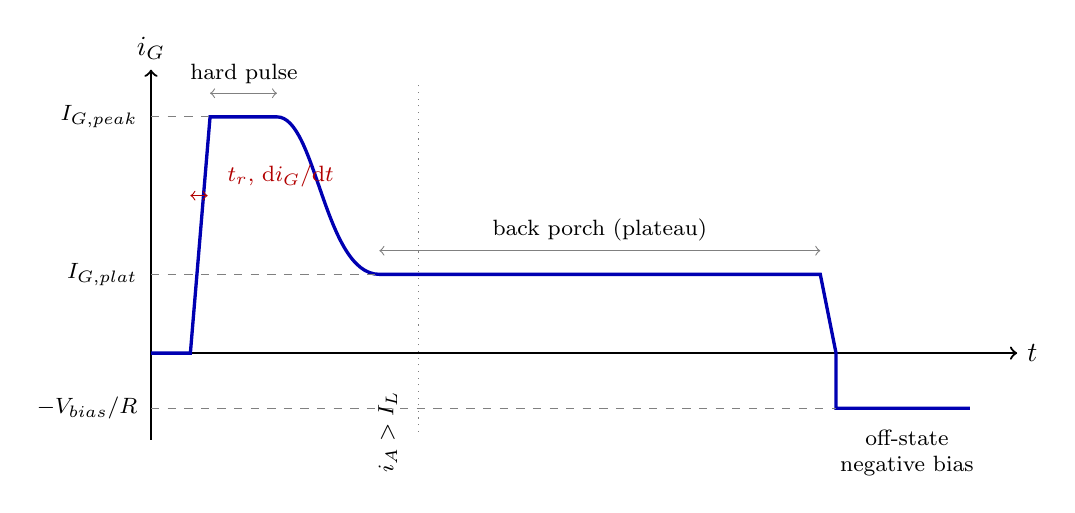
\begin{tikzpicture}[xscale=1.0,yscale=1.0]
  \draw[->,thick] (0,0) -- (11,0) node[right] {$t$};
  \draw[->,thick] (0,-1.1) -- (0,3.6) node[above] {$i_G$};

  % waveform
  \draw[very thick,blue!70!black]
    (0,0) -- (0.5,0) -- (0.75,3.0) -- (1.6,3.0)
    .. controls (2.1,3.0) and (2.2,1.0) .. (2.9,1.0)
    -- (8.5,1.0) -- (8.7,0) -- (8.7,-0.7) -- (10.4,-0.7);

  % annotations
  \draw[<->,gray] (0.75,3.3) -- (1.6,3.3);
  \node[font=\footnotesize,anchor=south] at (1.18,3.3) {hard pulse};
  \draw[<->,gray] (2.9,1.3) -- (8.5,1.3);
  \node[font=\footnotesize,anchor=south] at (5.7,1.3) {back porch (plateau)};
  \draw[dashed,gray] (0,3.0) -- (0.75,3.0);
  \node[font=\footnotesize,anchor=east] at (-0.05,3.0) {$I_{G,\text{peak}}$};
  \draw[dashed,gray] (0,1.0) -- (2.9,1.0);
  \node[font=\footnotesize,anchor=east] at (-0.05,1.0) {$I_{G,\text{plat}}$};
  \draw[dashed,gray] (0,-0.7) -- (8.7,-0.7);
  \node[font=\footnotesize,anchor=east] at (-0.05,-0.7) {$-V_{bias}/R$};
  \node[font=\footnotesize,anchor=north,align=center] at (9.6,-0.85)
    {off-state\\negative bias};
  % rise time
  \draw[<->,red!70!black] (0.5,2.0) -- (0.72,2.0);
  \node[font=\footnotesize,anchor=west,red!70!black] at (0.85,2.25)
    {$t_r$, $\mathrm{d}i_G/\mathrm{d}t$};
  % latching
  \draw[dotted,gray] (3.4,-1.0) -- (3.4,3.4);
  \node[font=\footnotesize,anchor=south,rotate=90] at (3.25,-1.0)
    {$i_A > I_L$};
\end{tikzpicture}
\caption{Recommended gate current waveform: a hard initial pulse for fast,
large-area turn-on, a back porch that holds the device until latching, and a
negative (or zero) bias in the off state.}
\label{thygate:fig:pulse}
\end{figure}

\subsection{Off-state bias and \texorpdfstring{$\mathrm{d}v/\mathrm{d}t$}{dv/dt} immunity}

When the thyristor is off but forward biased, the displacement current through the
blocking junction capacitance, $i = C_j\,\mathrm{d}v/\mathrm{d}t$, flows partly
into the gate region and can trigger the device. Countermeasures, in order of
effectiveness:

\begin{enumerate}
  \item A \textbf{gate--cathode resistor} $R_{GK}$ mounted \emph{at the device},
        typically \SIrange{10}{100}{\ohm} for large devices and up to
        \SI{1}{\kilo\ohm} for small ones. It diverts the displacement current and
        the junction leakage away from the gate. It also loads the driver, and this
        must be included in the sizing.
  \item A \textbf{negative gate bias} of \SIrange{-2}{-5}{\volt} between pulses.
        This is the most robust solution but requires a bipolar output stage and
        must respect $V_{RGM}$ with margin, including all ringing.
  \item A \textbf{low-impedance off state}: the output stage must present a low
        impedance to the gate when idle, not a high impedance.
\end{enumerate}

Note that snubber design and $\mathrm{d}v/\mathrm{d}t$ immunity are coupled: a
gate unit cannot compensate for an inadequate RC snubber.

\subsection{Summary of target values}

\begin{table}[htbp]
\centering
\caption{Typical design targets for a phase-control thyristor gate driver.
Datasheet values always override these figures.}
\label{thygate:tab:targets}
\begin{tabular}{@{}llp{6.4cm}@{}}
\toprule
\textbf{Quantity} & \textbf{Typical target} & \textbf{Remark} \\
\midrule
$I_{G,\text{peak}}$ & $3\dots10\times I_{GT}(T_{\min})$ &
  Upper end for high $\mathrm{d}i/\mathrm{d}t$ \\
$\mathrm{d}i_G/\mathrm{d}t$ & \SIrange{1}{5}{\ampere\per\micro\second} &
  Measured at the device terminals \\
$t_r$ & \SIrange{0.1}{1}{\micro\second} & Sets the gate loop inductance budget \\
Hard pulse width & \SIrange{10}{50}{\micro\second} & Covers turn-on delay and spreading \\
$I_{G,\text{plat}}$ & $1\dots2\times I_{GT}$ & Limited by $P_{G(AV)}$ \\
Plateau duration & until $i_A > I_L$ &
  Whole conduction interval for inductive loads \\
Off-state bias & \SI{0}{\volt} to \SI{-5}{\volt} &
  Never exceed $V_{RGM}$, ringing included \\
$R_{GK}$ & \SIrange{10}{100}{\ohm} & Mounted at the device, not at the driver \\
Jitter & $< \SI{1}{\micro\second}$ &
  Critical for series stacks and current sharing \\
Command-to-gate delay & matched within \SI{1}{\micro\second} &
  Across all channels of a bridge \\
\bottomrule
\end{tabular}
\end{table}

%======================================================================
\section{Isolation and Insulation Coordination}
%======================================================================

The gate unit straddles the main insulation barrier of the converter, and its
insulation rating must be derived from the same coordination study as the rest of
the equipment (IEC 60664-1, IEC 61800-5-1 for drives), considering:

\begin{itemize}
  \item the \textbf{steady-state common-mode voltage} of the cathode with respect
        to control ground;
  \item the \textbf{repetitive peak} and the \textbf{impulse withstand} levels
        (BIL) of the installation;
  \item \textbf{creepage and clearance} for the pollution degree and altitude of
        the site;
  \item \textbf{partial discharge inception voltage} for medium-voltage equipment,
        which usually governs the design of the isolation transformer well before
        the dielectric withstand does;
  \item the \textbf{common-mode transient immunity} (CMTI), i.e.\ the
        $\mathrm{d}v/\mathrm{d}t$ that the barrier sees during commutation. The
        coupling capacitance across the barrier, $C_{io}$, injects
        $i = C_{io}\,\mathrm{d}v/\mathrm{d}t$ into the control electronics.
        Minimising $C_{io}$ (electrostatic shield between windings, fibre optics)
        is the primary defence.
\end{itemize}

Three isolation strategies are used:

\begin{table}[htbp]
\centering
\caption{Comparison of isolation strategies for the firing command.}
\label{thygate:tab:iso}
\begin{tabular}{@{}p{3.1cm}p{4.6cm}p{4.6cm}@{}}
\toprule
\textbf{Strategy} & \textbf{Advantages} & \textbf{Limitations} \\
\midrule
Pulse transformer &
  Carries command and energy together; no local supply needed; simple, robust,
  proven &
  Volt-second limit constrains pulse length; leakage inductance limits
  $\mathrm{d}i_G/\mathrm{d}t$; core reset required; $C_{io}$ of the order of
  \si{\pico\farad} \\
\addlinespace
Optocoupler + isolated supply &
  Arbitrary pulse length; easy shaping; low cost &
  Isolation typically limited to a few \si{\kilo\volt}; CMTI is a design
  constraint; requires an isolated auxiliary supply \\
\addlinespace
Fibre optic + local supply &
  Essentially unlimited isolation; negligible $C_{io}$; ideal for series stacks
  and MV &
  Requires a local energy source (auxiliary transformer or self-powering);
  more components; fibre handling and ageing \\
\bottomrule
\end{tabular}
\end{table}

For series-connected stacks, fibre optics is effectively mandatory, both for the
insulation level and because the transmission delay must be matched across all
levels to within a microsecond to avoid unequal voltage sharing during turn-on.

%======================================================================
\section{Auxiliary Power for the Gate Unit}
%======================================================================

The gate unit consumes, per firing, an energy of the order

\begin{equation}
  E_{fire} \approx V_G I_{G,\text{peak}} t_{hard} + V_G I_{G,\text{plat}} t_{plat},
\end{equation}

which for a large device is a few millijoules --- small in absolute terms, but it
must be available with a low source impedance to satisfy
Eq.~\eqref{thygate:eq:didt}. Options:

\begin{enumerate}
  \item \textbf{Isolated DC/DC converter} with a high-isolation transformer feeding
        the floating side. Straightforward, but the transformer becomes the
        insulation-critical component and its inter-winding capacitance directly
        degrades CMTI.
  \item \textbf{Auxiliary winding on the main transformer} or a dedicated
        low-power potential transformer, common in large phase-control rectifiers.
  \item \textbf{Self-powering from the anode--cathode voltage}, harvesting energy
        during the blocking interval through a high-voltage series resistor or,
        more efficiently, from the RC snubber current. This removes the barrier
        entirely for the power path, but requires careful start-up handling, since
        no energy is available before the converter is energised.
  \item \textbf{Local storage capacitor} sized for several consecutive pulses, so
        that the pulse current is drawn from the capacitor and not from the supply.
        This is what actually determines the achievable
        $\mathrm{d}i_G/\mathrm{d}t$: place the capacitor immediately at the output
        stage.
\end{enumerate}

%======================================================================
\section{Circuit Proposals}
%======================================================================

Four topologies are proposed, in increasing order of capability and cost.

\subsection{Circuit A --- Pulse transformer with peaking network}

This is the reference solution for single devices and short-to-medium pulses
(Fig.~\ref{thygate:fig:circA}). A low-side MOSFET applies the auxiliary rail to the
transformer primary. The DC blocking capacitor $C_b$ provides automatic core reset
and blocks any DC component caused by a stuck-on driver, which would otherwise
saturate the core and destroy the MOSFET.

On the secondary, the peaking network shapes the two-level waveform of
Fig.~\ref{thygate:fig:pulse}: at the leading edge $C_p$ short-circuits $R_p$, so the gate
current is limited only by $R_s$ and the peak value is high; as $C_p$ charges, the
current settles to the plateau value set by $R_s + R_p$. Design equations:

\begin{align}
  I_{G,\text{peak}} &\approx \frac{n V_{cc} - V_{GT} - V_{D}}{R_s},
  &
  I_{G,\text{plat}} &\approx \frac{n V_{cc} - V_{GT} - V_{D}}{R_s + R_p}
      - \frac{V_{GT}}{R_{GK}},
  \label{thygate:eq:peak}\\[1mm]
  \tau_p &= C_p\,\big(R_p \parallel R_s\big),
  &
  t_{hard} &\approx 3\tau_p ,
\end{align}

where $n$ is the turns ratio and $V_D$ the drop of the series blocking diode $D_s$.
The volt-second capability of the core sets the maximum pulse length:

\begin{equation}
  A_e \;\ge\; \frac{V_{cc}\, t_{pulse}}{N_1 \Delta B}.
  \label{thygate:eq:volt-sec}
\end{equation}

\begin{figure}[htbp]
\centering
\begin{circuitikz}[american]
  % ---------- primary side ----------
  \draw (0.0,6.4) node[left,font=\small]{$+V_{cc}$} -- (1.0,6.4);
  \draw (1.0,6.4) to[C, l_=$C_{st}$, *-] (1.0,3.2) node[ground]{};
  \draw (1.0,6.4) to[C, l=$C_b$] (2.6,6.4);
  \draw (2.6,6.4) -- (5.0,6.4);
  \draw (3.4,6.4) to[zzD, l_=$D_z$, *-] (3.4,3.6);
  \draw (3.4,3.6) -- (4.2,3.6);
  % transformer
  \node[transformer core] (T) at (5.8,5.0) {};
  \draw (5.0,6.4) -| (T.A1);
  \draw (T.A2) -| (4.2,3.6);
  % primary switch
  \node[nigfete, anchor=D] (M) at (4.2,3.6) {};
  \fill (4.2,3.6) circle (1.6pt);
  \draw (M.S) -- (4.2,1.9) node[ground]{};
  \draw (M.G) -- ++(-0.3,0) to[R, l_=$R_g$] ++(-0.6,0)
        node[left,font=\scriptsize]{firing cmd};
  % isolation barrier
  \draw[dashed,gray] (5.8,1.9) -- (5.8,4.1);
  \draw[dashed,gray] (5.8,5.9) -- (5.8,7.9);
  \node[gray!50!black,font=\footnotesize] at (5.8,1.5) {isolation barrier};
  % ---------- secondary side ----------
  \draw (T.B1) -| (7.2,6.4);
  \draw (7.2,6.4) to[D, l=$D_s$] (8.4,6.4);
  \draw (8.4,6.4) to[R, l=$R_s$] (9.7,6.4);
  \draw (10.0,6.4) to[R, l_=$R_p$] (11.4,6.4);
  \draw (9.7,6.4) -- (10.0,6.4);
  \draw (10.0,6.4) -- (10.0,7.5) to[C, l=$C_p$] (11.4,7.5) -- (11.4,6.4);
  \draw (11.4,6.4) -- (13.4,6.4);
  % return conductor
  \draw (T.B2) -| (7.2,2.6);
  \draw (7.2,2.6) -- (13.9,2.6);
  % network at the device terminals
  \draw (11.9,6.4) to[R, l_=$R_{GK}$, *-*] (11.9,2.6);
  \draw (12.9,6.4) to[zzD, *-*] (12.9,2.6);
  \node[font=\footnotesize] at (12.9,6.85) {$D_{tvs}$};
  % thyristor
  \draw (13.9,7.9) node[above,font=\footnotesize]{A} -- (13.9,7.4);
  \draw (13.9,7.4) to[Ty, mirror, n=Th, l=$Th$] (13.9,3.4);
  \draw (13.9,3.4) -- (13.9,2.0) node[below,font=\footnotesize]{K};
  \draw (Th.G) -| (13.4,6.4);
  \fill (13.9,2.6) circle (1.6pt);
\end{circuitikz}
\caption{Circuit A --- pulse transformer gate driver with DC blocking capacitor
$C_b$ for core reset, primary clamp $D_z$, and secondary peaking network
$R_s$/$R_p$/$C_p$ producing the hard-pulse-plus-back-porch waveform. $R_{GK}$ and
the TVS are mounted at the device terminals.}
\label{thygate:fig:circA}
\end{figure}

\paragraph{Notes.}
\begin{itemize}
  \item The series diode $D_s$ prevents reverse gate current during core reset and
        protects the gate against the negative excursion; without it, $V_{RGM}$ is
        easily exceeded.
  \item The leakage inductance of the transformer appears in series with the gate
        loop and directly limits $\mathrm{d}i_G/\mathrm{d}t$. Bifilar or
        interleaved winding is required; but interleaving increases $C_{io}$, so
        the two requirements must be traded off explicitly.
  \item The local storage capacitor $C_{st}$ must be placed at the primary of the
        transformer, with minimum loop area to the MOSFET.
\end{itemize}

\subsection{Circuit B --- Chopped (pulse-train) driver}

Equation~\eqref{thygate:eq:volt-sec} makes long pulses expensive: a \SI{500}{\micro\second}
pulse at \SI{24}{\volt} requires a core roughly twenty times larger than a
\SI{25}{\micro\second} pulse. The standard solution is to \emph{chop} the pulse at
\SIrange{5}{20}{\kilo\hertz} (Fig.~\ref{thygate:fig:circB}). The transformer then only sees
the volt-seconds of one carrier period, while the envelope can be arbitrarily long.

\begin{figure}[htbp]
\centering
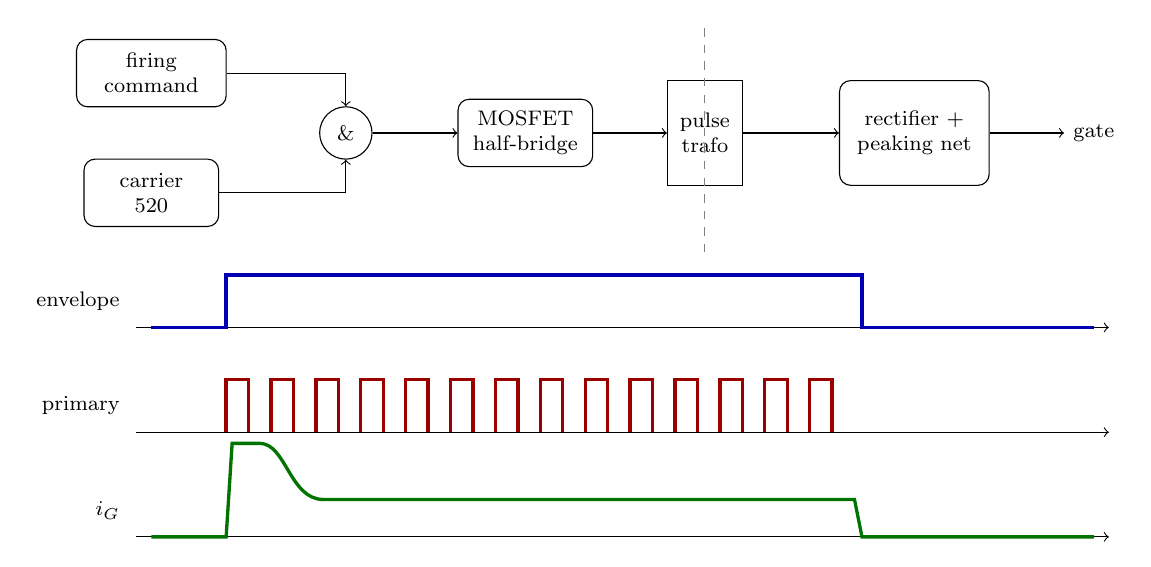
\begin{tikzpicture}[scale=0.95,transform shape]
  % block diagram
  \node[draw,rounded corners,minimum width=2.0cm,minimum height=0.9cm,align=center,font=\footnotesize]
    (cmd) at (0,0) {firing\\command};
  \node[draw,rounded corners,minimum width=1.8cm,minimum height=0.9cm,align=center,font=\footnotesize]
    (osc) at (0,-1.6) {carrier\\\SIrange{5}{20}{\kilo\hertz}};
  \node[draw,circle,minimum size=0.7cm,font=\footnotesize] (and) at (2.6,-0.8) {\&};
  \node[draw,rounded corners,minimum width=1.8cm,minimum height=0.9cm,align=center,font=\footnotesize]
    (drv) at (5.0,-0.8) {MOSFET\\half-bridge};
  \node[draw,minimum width=1.0cm,minimum height=1.4cm,align=center,font=\footnotesize]
    (tr) at (7.4,-0.8) {pulse\\trafo};
  \node[draw,rounded corners,minimum width=2.0cm,minimum height=1.4cm,align=center,font=\footnotesize]
    (rect) at (10.2,-0.8) {rectifier +\\peaking net};
  \node[font=\footnotesize] (th) at (12.6,-0.8) {gate};

  \draw[->] (cmd) -| (and);
  \draw[->] (osc) -| (and);
  \draw[->] (and) -- (drv);
  \draw[->] (drv) -- (tr);
  \draw[->] (tr) -- (rect);
  \draw[->] (rect) -- (th);
  \draw[dashed,gray] (7.4,0.6) -- (7.4,-2.4);

  % waveforms
  \begin{scope}[shift={(0,-3.4)}]
    \draw[->] (-0.2,0) -- (12.8,0);
    \node[font=\footnotesize,anchor=east] at (-0.3,0.35) {envelope};
    \draw[very thick,blue!70!black]
      (0,0) -- (1.0,0) -- (1.0,0.7) -- (9.5,0.7) -- (9.5,0) -- (12.6,0);
  \end{scope}
  \begin{scope}[shift={(0,-4.8)}]
    \draw[->] (-0.2,0) -- (12.8,0);
    \node[font=\footnotesize,anchor=east] at (-0.3,0.35) {primary};
    \foreach \x in {1.0,1.6,...,9.2} {
      \draw[very thick,red!60!black] (\x,0) -- (\x,0.7) -- (\x+0.3,0.7) -- (\x+0.3,0);
    }
  \end{scope}
  \begin{scope}[shift={(0,-6.2)}]
    \draw[->] (-0.2,0) -- (12.8,0);
    \node[font=\footnotesize,anchor=east] at (-0.3,0.35) {$i_G$};
    \draw[very thick,green!45!black]
      (0,0) -- (1.0,0) -- (1.08,1.25) -- (1.45,1.25)
      .. controls (1.8,1.25) and (1.85,0.5) .. (2.3,0.5)
      -- (9.4,0.5) -- (9.5,0) -- (12.6,0);
  \end{scope}
\end{tikzpicture}
\caption{Circuit B --- chopped gate driver. The firing envelope is modulated by a
\SIrange{5}{20}{\kilo\hertz} carrier so that the transformer only handles the
volt-seconds of a single carrier period. Light filtering on the secondary
reconstructs a quasi-continuous gate current.}
\label{thygate:fig:circB}
\end{figure}

The secondary filtering must be a compromise: enough capacitance to smooth the
plateau between carrier pulses, little enough not to slow the leading edge. A
common arrangement is a fast rectifier feeding the peaking network of Circuit~A,
with a small filter capacitor placed \emph{after} the peaking network. A half-bridge
(or full-bridge) primary is preferred over a single-ended stage, since it doubles
the usable flux swing and provides intrinsic core reset.

\subsection{Circuit C --- Fibre-optic gate unit with two-level current source}

For medium-voltage equipment and series stacks, the command is transmitted over
plastic optical fibre and the energy is stored locally (Fig.~\ref{thygate:fig:circC}). The
output stage is a two-level source: $M_1$ delivers the hard pulse from the storage
capacitor $C_{st}$ through the low resistance $R_1$; a monostable then releases
$M_1$ and $M_2$ maintains the plateau through $R_2$ for as long as the optical
command is present. Between pulses $M_3$ applies the negative bias and holds the
gate at low impedance.

\begin{figure}[htbp]
\centering
\begin{circuitikz}[american]
  % fibre receiver and logic
  \draw[->,very thick,orange!80!black] (0.0,4.4) -- (0.85,4.4);
  \node[font=\footnotesize,anchor=south] at (0.42,4.5) {POF};
  \node[draw,rounded corners,minimum width=2.6cm,minimum height=1.5cm,
        align=center,font=\footnotesize] (lg) at (2.2,4.4)
        {fibre rx\\pulse shaper\\+ monostable};
  \draw[->,thick] (3.5,4.4) -- (4.6,4.4);
  \node[font=\scriptsize,anchor=south] at (4.05,4.78) {gate signals};
  % output stage boundary
  \draw[dashed,gray!70] (4.75,0.85) rectangle (13.85,7.45);
  \node[gray!50!black,font=\footnotesize,anchor=south west] at (4.85,0.95)
        {output stage --- floating, referenced to K};
  % rails
  \draw (5.0,6.6) node[left,font=\small]{$+V_{cc}$} -- (11.9,6.6);
  \draw (5.3,6.6) to[C, l=$C_{st}$, *-] (5.3,1.6);
  \draw (5.3,1.6) -- (14.2,1.6);
  % M1 : hard pulse branch
  \node[pigfete, anchor=S] (M1) at (7.6,6.6) {};
  \draw (M1.D) to[R, l=$R_1$] (7.6,4.4);
  \draw (M1.G) -- ++(-0.4,0) node[left,font=\scriptsize]{hard};
  \node[font=\footnotesize,anchor=west] at (7.9,5.7) {$M_1$};
  % M2 : plateau branch
  \node[pigfete, anchor=S] (M2) at (9.9,6.6) {};
  \draw (M2.D) to[R, l=$R_2$] (9.9,4.4);
  \draw (M2.G) -- ++(-0.4,0) node[left,font=\scriptsize]{plateau};
  \node[font=\footnotesize,anchor=west] at (10.2,5.7) {$M_2$};
  % summing node
  \draw (7.6,4.4) -- (13.8,4.4);
  \fill (9.9,4.4) circle (1.6pt);
  \fill (11.6,4.4) circle (1.6pt);
  % M3 : off-state negative bias
  \node[nigfete, anchor=D] (M3) at (11.6,4.4) {};
  \draw (M3.S) -- (11.6,2.6);
  \draw (11.25,2.6) -- (11.95,2.6);
  \node[font=\footnotesize,anchor=north] at (11.6,2.5) {$-V_b$};
  \draw (M3.G) -- ++(-0.5,0) node[left,font=\scriptsize]{off bias};
  \node[font=\footnotesize,anchor=west] at (11.95,3.95) {$M_3$};
  % device-side network
  \draw (12.6,4.4) to[R, l_=$R_{GK}$, *-*] (12.6,1.6);
  \draw (13.4,4.4) to[zzD, *-*] (13.4,1.6);
  % thyristor
  \draw (14.2,6.9) node[above,font=\footnotesize]{A} -- (14.2,6.6);
  \draw (14.2,6.6) to[Ty, mirror, n=Th] (14.2,2.8);
  \draw (14.2,2.8) -- (14.2,1.0) node[below,font=\footnotesize]{K};
  \draw (Th.G) -| (13.8,4.4);
  \fill (14.2,1.6) circle (1.6pt);
\end{circuitikz}
\caption{Circuit C --- fibre-optic gate unit with local storage and a two-level
output stage. $M_1$ sources the hard pulse through $R_1$, $M_2$ the back porch
through $R_2$, and $M_3$ applies the negative off-state bias.}
\label{thygate:fig:circC}
\end{figure}

\paragraph{Notes.}
\begin{itemize}
  \item $C_{st}$ must be a low-ESL type placed within a few millimetres of $M_1$;
        it, and not the auxiliary supply, determines the achievable
        $\mathrm{d}i_G/\mathrm{d}t$.
  \item The monostable that terminates the hard pulse should be retriggerable and
        should have a defined maximum on-time, so that a stuck-high optical input
        cannot exceed $P_{G(AV)}$.
  \item A watchdog on the optical link is essential: loss of fibre must be
        interpreted as ``no fire'', never as ``fire''. Use a modulated optical
        carrier rather than a static light level so that a broken fibre and a
        permanent-off command are distinguishable.
\end{itemize}

\subsection{Circuit D --- Self-powered gate unit}

Where no auxiliary supply is available on the floating side --- typically in
high-voltage series stacks --- the gate unit harvests its energy from the
anode--cathode voltage (Fig.~\ref{thygate:fig:circD}). A high-voltage current-limiting
network in parallel with the snubber charges the local storage capacitor during the
blocking interval; a shunt regulator clamps the storage voltage. The fibre carries
only the command.

\begin{figure}[htbp]
\centering
\begin{circuitikz}[american]
  % ---------- rails ----------
  \draw (2.0,4.6) -- (10.6,4.6);
  \node[font=\footnotesize,anchor=south] at (5.9,4.65) {$+V_{cc}$};
  \draw (2.0,1.4) -- (13.2,1.4);
  % ---------- fibre receiver and logic ----------
  \draw[->,very thick,orange!80!black] (0.4,3.0) -- (2.1,3.0);
  \node[font=\footnotesize,anchor=south] at (1.25,3.1) {POF};
  \node[draw,rounded corners,minimum width=2.2cm,minimum height=1.3cm,
        align=center,font=\footnotesize] (lg) at (3.2,3.0) {fibre rx\\+ logic};
  \draw (3.2,3.65) -- (3.2,4.6);
  \draw (3.2,2.35) -- (3.2,1.4);
  \draw[->,dashed,gray!60!black] (4.3,3.0) -- (8.9,3.0);
  % ---------- storage and shunt regulator ----------
  \draw (6.8,4.6) to[zD, invert, *-*] (6.8,1.4);
  \node[font=\footnotesize,anchor=south east] at (6.7,3.75) {$D_{sh}$};
  \draw (8.2,4.6) to[C, *-*] (8.2,1.4);
  \node[font=\footnotesize,anchor=south east] at (8.1,3.75) {$C_{st}$};
  % ---------- output stage ----------
  \node[draw,rounded corners,minimum width=2.4cm,minimum height=1.2cm,
        align=center,font=\footnotesize] (out) at (10.2,3.0) {two-level\\output stage};
  \draw (10.2,3.6) -- (10.2,4.6);
  \draw (10.2,2.4) -- (10.2,1.4);
  % ---------- harvesting branch ----------
  \draw (13.2,6.8) -- (10.6,6.8);
  \draw (10.6,6.8) to[R, l_=$R_h$] (10.6,5.6);
  \draw (10.6,5.6) to[D, l_=$D_h$] (10.6,4.6);
  % ---------- gate network ----------
  \draw (11.4,3.0) -- (12.0,3.0) -- (12.0,4.4) -- (12.6,4.4);
  \draw (12.6,4.4) to[R, *-*] (12.6,1.4);
  \node[font=\footnotesize,anchor=east] at (12.3,2.5) {$R_{GK}$};
  % ---------- thyristor ----------
  \draw (13.2,7.3) node[above,font=\footnotesize]{A} -- (13.2,6.8);
  \draw (13.2,6.8) to[Ty, mirror, n=Th] (13.2,3.0);
  \draw (13.2,3.0) -- (13.2,0.9) node[below,font=\footnotesize]{K};
  \draw (Th.G) -| (12.6,4.4);
  \fill (13.2,6.8) circle (1.6pt);
  \fill (13.2,1.4) circle (1.6pt);
  % ---------- snubber ----------
  \draw (13.2,6.8) -- (14.6,6.8);
  \draw (14.6,6.8) to[R, l=$R_{sn}$] (14.6,4.8);
  \draw (14.6,4.8) to[C, l=$C_{sn}$] (14.6,2.0);
  \draw (14.6,2.0) -- (13.2,2.0);
  \fill (13.2,2.0) circle (1.6pt);
\end{circuitikz}
\caption{Circuit D --- self-powered gate unit. Energy is harvested from the
anode--cathode blocking voltage through $R_h$/$D_h$ and stored in $C_{st}$, clamped
by the shunt regulator $D_{sh}$. No auxiliary supply crosses the insulation
barrier.}
\label{thygate:fig:circD}
\end{figure}

\paragraph{Notes.}
\begin{itemize}
  \item Start-up must be handled explicitly: the first firing after energisation
        can only occur once $C_{st}$ is charged. Either the control must wait for a
        ``ready'' feedback, or the first cycles must be fired in a mode that does
        not require full gate energy.
  \item $R_h$ dissipates continuously in the blocking state and must be rated for
        the full repetitive peak voltage. Harvesting from the snubber current
        instead of a resistive divider is considerably more efficient.
  \item In a series stack, the harvesting network is part of the static and dynamic
        voltage-sharing design and must be included in the sharing calculation.
\end{itemize}

%======================================================================
\section{Protection, Layout and EMC}
%======================================================================

\subsection{Component-level protection}

\begin{itemize}
  \item \textbf{$R_{GK}$ at the device.} Mandatory. Placed on the device terminals,
        not on the driver board.
  \item \textbf{Reverse-voltage protection.} A series diode or an anti-parallel
        diode limits the negative gate excursion. $V_{RGM}$ of a few volts is
        easily exceeded by ringing in a long gate cable.
  \item \textbf{Bidirectional TVS} across gate and cathode, at the device, for
        transients coupled into the gate loop. Its clamping voltage must sit
        between the drive voltage and $V_{FGM}$/$V_{RGM}$.
  \item \textbf{Series gate resistance.} Beyond setting the current level, it damps
        the resonance between the gate loop inductance and the device gate
        capacitance and prevents oscillatory retriggering.
  \item \textbf{Output stage current limit or fuse} on the driver side, so that a
        short-circuited gate lead does not destroy the gate unit.
\end{itemize}

\subsection{Gate loop layout}

\begin{itemize}
  \item Use a \textbf{twisted pair} for the gate--cathode connection; a shielded
        twisted pair, with the shield bonded at the driver end only, if the
        environment is harsh. Both conductors must be routed together over the
        entire length --- a common error is to take the cathode return from a power
        terminal.
  \item Keep the \textbf{loop area} minimal. The gate loop is a receiving antenna
        for the $\mathrm{d}i/\mathrm{d}t$ of the main circuit.
  \item Keep the \textbf{cable length} within the budget of
        Eq.~\eqref{thygate:eq:lloop}. Below \SI{1}{\metre} is preferable; beyond a few
        metres the peaking network must be redesigned or the drive voltage raised.
  \item \textbf{Route the gate cable away from the main busbars} and cross them at
        right angles where crossing cannot be avoided.
  \item In a bridge, keep the \textbf{propagation delay matched} across all
        channels; a mismatch translates directly into unequal voltage sharing in
        series connections and unequal current sharing in parallel connections.
\end{itemize}

\subsection{Common-mode considerations}

The barrier capacitance $C_{io}$ and the commutation $\mathrm{d}v/\mathrm{d}t$
define a common-mode current that returns through the control ground. Design
measures: electrostatic shield in the isolation transformer connected to the
control ground; common-mode chokes on the primary leads; fibre optics where the
$\mathrm{d}v/\mathrm{d}t$ is severe. Verify by direct measurement with a
common-mode transient generator rather than by calculation.

%======================================================================
\section{Diagnostics and Feedback}
%======================================================================

In industrial equipment the gate unit is usually expected to provide at least:

\begin{itemize}
  \item \textbf{Pulse confirmation} --- a feedback signal indicating that the gate
        current pulse actually flowed, obtained from a small current transformer or
        a shunt in the gate loop. This distinguishes a driver fault from a device
        fault.
  \item \textbf{Anode voltage monitoring} --- a divider indicating whether the
        device is blocking or conducting. Used for turn-on verification, for
        detecting a shorted device before energisation, and for missing-pulse
        detection.
  \item \textbf{Supply undervoltage lockout} --- inhibits firing when the local
        supply is below the level needed to meet the drive specification. Firing
        with insufficient gate current is more damaging than not firing at all,
        because turn-on occurs over a small area.
  \item \textbf{Overtemperature and watchdog} on the gate unit itself.
\end{itemize}

For series stacks, the pulse confirmation signals of all levels should be combined
into a single ``stack healthy'' indication, since a single missing pulse imposes
the whole stack voltage on one device.

%======================================================================
\section{Worked Example}
%======================================================================

Consider a large press-pack phase-control thyristor, roughly
\SI{6.5}{\kilo\volt}/\SI{2.6}{\kilo\ampere}, in a six-pulse line-commutated bridge
with an inductive load. Representative datasheet values (to be replaced by the
actual ones):

\begin{center}
\begin{tabular}{@{}lll@{}}
\toprule
$I_{GT}$ at \SI{25}{\celsius} & \SI{250}{\milli\ampere} & max \\
$I_{GT}$ at \SI{-40}{\celsius} & \SI{600}{\milli\ampere} & estimated, $\approx 2.5\times$ \\
$V_{GT}$ & \SI{3}{\volt} & max \\
$V_{GD}$ / $I_{GD}$ at $T_{vj,\max}$ & \SI{0.25}{\volt} / \SI{10}{\milli\ampere} & \\
$I_L$ & \SI{2}{\ampere} & \\
$V_{FGM}$ / $I_{FGM}$ / $V_{RGM}$ & \SI{10}{\volt} / \SI{8}{\ampere} / \SI{5}{\volt} & \\
$P_{GM}$ / $P_{G(AV)}$ & \SI{100}{\watt} / \SI{15}{\watt} & \\
\bottomrule
\end{tabular}
\end{center}

\paragraph{Step 1 --- Pulse amplitude.}
From Eq.~\eqref{thygate:eq:amp} with $I_{GT}(T_{\min}) = \SI{0.6}{\ampere}$ and a factor of
5: $I_{G,\text{peak}} = \SI{3}{\ampere}$, comfortably below $I_{FGM}$.
Peak gate power $\approx \SI{5}{\volt}\times\SI{3}{\ampere} = \SI{15}{\watt}$,
well below $P_{GM}$.

\paragraph{Step 2 --- Plateau.}
$I_{G,\text{plat}} = 1.5\times I_{GT}(\SI{25}{\celsius}) \approx
\SI{0.9}{\ampere}$. With a conduction interval of \SI{6.7}{\milli\second} at
\SI{50}{\hertz}, the duty over a \SI{20}{\milli\second} window is $1/3$, hence
$P_{G(AV)} \approx \SI{3.5}{\volt}\times\SI{0.9}{\ampere}\times 1/3 \approx
\SI{1.1}{\watt}$, acceptable.

\paragraph{Step 3 --- Peaking network.}
Take $V_{drive} = \SI{15}{\volt}$ and $V_{GT}+V_{D} = \SI{3.5}{\volt}$, so
\SI{11.5}{\volt} is available. From Eq.~\eqref{thygate:eq:peak}:
\[
  R_s = \frac{\SI{11.5}{\volt}}{\SI{3}{\ampere}} \approx \SI{4}{\ohm},
  \qquad
  R_s + R_p = \frac{\SI{11.5}{\volt}}{\SI{0.9}{\ampere} + \SI{0.11}{\ampere}}
  \approx \SI{11.4}{\ohm} \Rightarrow R_p \approx \SI{7.5}{\ohm},
\]
where \SI{0.11}{\ampere} is the current diverted by $R_{GK} = \SI{27}{\ohm}$ at
\SI{3}{\volt}. For a hard-pulse duration of \SI{20}{\micro\second}:
\[
  \tau_p = \frac{t_{hard}}{3} \approx \SI{6.7}{\micro\second},
  \qquad
  C_p = \frac{\tau_p}{R_p \parallel R_s}
      = \frac{\SI{6.7}{\micro\second}}{\SI{2.6}{\ohm}} \approx \SI{2.6}{\micro\farad}
      \;\rightarrow\; \SI{2.2}{\micro\farad}.
\]

\paragraph{Step 4 --- Gate loop inductance.}
Requiring $\mathrm{d}i_G/\mathrm{d}t = \SI{3}{\ampere\per\micro\second}$ and using
Eq.~\eqref{thygate:eq:lloop} with the full \SI{11.5}{\volt} available at $t=0^+$:
\[
  L_{loop} \le \frac{\SI{11.5}{\volt}}{\SI{3}{\ampere\per\micro\second}}
  \approx \SI{3.8}{\micro\henry}.
\]
At \SI{1}{\micro\henry\per\metre} for a twisted pair, and reserving
\SI{1.5}{\micro\henry} for the transformer leakage and the layout, the cable is
limited to roughly \SI{2}{\metre}. Longer runs require either a higher drive
voltage or a local gate unit.

\paragraph{Step 5 --- Transformer core.}
For a directly transmitted pulse of \SI{500}{\micro\second} at \SI{24}{\volt} with
$N_1 = 20$ and $\Delta B = \SI{0.3}{\tesla}$, Eq.~\eqref{thygate:eq:volt-sec} gives
$A_e \ge \SI{2000}{\milli\metre\squared}$ --- impractical. Chopping at
\SI{20}{\kilo\hertz} with \SI{50}{\percent} duty reduces the requirement to
$A_e \ge \SI{100}{\milli\metre\squared}$, an ordinary small core. This single
calculation is the reason Circuit~B is the standard choice whenever long pulses
are needed.

%======================================================================
\section{Design Checklist}
%======================================================================

\begin{enumerate}
  \item Datasheet limits collected: $I_{GT}$, $V_{GT}$ at $T_{vj,\min}$;
        $V_{GD}$, $I_{GD}$ at $T_{vj,\max}$; $I_L$, $I_H$; $V_{FGM}$, $I_{FGM}$,
        $V_{RGM}$; $P_{GM}$, $P_{G(AV)}$.
  \item Driver load line plotted on the trigger diagram and verified at both
        temperature extremes.
  \item $I_{G,\text{peak}}$ and $\mathrm{d}i_G/\mathrm{d}t$ consistent with the
        conditions under which the $\mathrm{d}i/\mathrm{d}t$ rating is specified.
  \item Pulse duration verified against the worst case: minimum load current,
        maximum load inductance, minimum supply voltage.
  \item $P_{G(AV)}$ verified at maximum firing frequency and maximum conduction
        angle.
  \item Off-state condition verified: $V_{GK} < V_{GD}$ at $T_{vj,\max}$, with
        $R_{GK}$ fitted.
  \item $V_{RGM}$ verified including ringing, measured at the device.
  \item Insulation: creepage, clearance, impulse withstand, partial discharge,
        $C_{io}$ and CMTI.
  \item Transformer volt-second capability verified at maximum pulse width,
        maximum supply voltage and maximum temperature; core reset mechanism
        present.
  \item Gate loop inductance budget verified against cable length.
  \item Undervoltage lockout, watchdog and fail-safe interpretation of a lost
        command.
  \item Channel-to-channel delay and jitter measured, not assumed.
  \item Verification performed on the actual device at the coldest specified
        temperature, with the weakest expected supply, and with the gate current
        measured \emph{at the device terminals}.
\end{enumerate}

%======================================================================
\section*{Notes on Verification}
\addcontentsline{toc}{section}{Notes on Verification}
%======================================================================

Two measurement practices are worth stating explicitly:

\begin{itemize}
  \item Measure the gate current with a current probe placed on the gate lead at
        the \emph{device}, and the gate voltage differentially at the \emph{device}
        terminals. What the driver output does is of secondary interest; the loop
        inductance and the cable are part of the circuit.
  \item Test at the extremes, not at nominal. A gate driver that works on the bench
        at \SI{25}{\celsius} with a new device and a short lead tells very little
        about behaviour at \SI{-25}{\celsius}, with a worst-case device and the
        installed cable length. Most field misfiring problems are traced to one of
        these three margins.
\end{itemize}

%======================================================================

